\section[Entropie statistique]{Entropie statistique}

\begin{frame}{Entropie statistique}
	Avant de parler des arbres de décision, nous allons faire un détour du côté du concept d'\textbf{entropie statistique} qui est clé:
	
	\begin{itemize}
		\item Pour les arbres de décision.
		\pause
		\item Pour la régression logistique comme nous l'avons déjà vu.
		\pause
		\item Mais aussi pour les réseaux de neurones qu'il nous reste à voir !
	\end{itemize}
\end{frame}

\subsection[Surprise]{Surprise}

\begin{frame}{Un exemple avec une pièce de monnaie}
	Prenons un exemple simple. Nous disposons d'une pièce de monnaie qui n'est pas équilibrée. Les probabilités d'obtenir "Face" ou "Pile" sur un lancé $X$ sont les suivantes:
	\begin{equation*}
		\begin{cases}
			P(X = \text{"Face"}) = 0 \\
			P(X = \text{"Pile"}) = 1
		\end{cases}
	\end{equation*}
	\pause
	\begin{itemize}
		\item J'effectue un lancé avec cette pièce et le résultat est "Pile".
		\item Rien de \textbf{surprenant} ici.
	\end{itemize}
\end{frame}

\begin{frame}{Un exemple avec une pièce de monnaie}
	Les probabilités de la pièce sont maintenant changées et nous avons ceci à la place:
	\begin{equation*}
		\begin{cases}
			P(X = \text{"Face"}) = 0.1 \\
			P(X = \text{"Pile"}) = 0.9
		\end{cases}
	\end{equation*}
	\pause
	\begin{itemize}
		\item J'effectue un lancé avec cette pièce et le résultat est "Pile".
		\item Ce n'est pas très surprenant comme résultat, mais un peu plus que dans l'exemple précédent tout de même.
	\end{itemize}
\end{frame}

\begin{frame}{Un exemple avec une pièce de monnaie}
	\begin{itemize}
		\item Moins la probabilité $P(X = \text{"Pile"})$ est forte, plus la \textbf{surprise} devient grande lorsque que le lancé aboutit sur "Pile".
		\pause
		\item Comment exprimer la surprise à partir de la probabilité ?
	\end{itemize}
	\pause
	Une première tentative pourrait être, en notant la surprise $I$:
	\begin{equation*}
		I(\text{"Pile"}) = \frac{1}{P(X = \text{"Pile"})}
	\end{equation*}
	\pause
	\begin{itemize}
		\item Plus la probabilité est faible et plus la surprise devient grande.
		\pause
		\item Mais si la probabilité $P(X = \text{"Pile"}) = 1$ alors la surprise est $I(\text{"Pile"}) = 1$.
		\pause
		\item Il semblerait plus naturel que la surprise soit nulle si l'événement est certain.
	\end{itemize}
\end{frame}

\begin{frame}{Surprise ou Information}
	\begin{block}{Définition: Surprise ou Information}
		Dans sa théorie de l'information, Claude Shannon a définit le concept de \textbf{surprise}, aussi appelée \textbf{information} et notée $I$, comme l'inverse du logarithme de la probabilité $P$ d'un événement $x$:
		\begin{equation*}
			I(x) = \ln{\left(\frac{1}{P(X = x)}\right)} = - \ln{P(X = x)}
		\end{equation*}
		Dans cette équation, $x$ représente la réalisation d'une variable aléatoire $X$.
		
		\vspace{0.3cm}
		\hfill
		\textit{--- Claude Shannon (1948)}
	\end{block}
	\pause
	Grâce à l'utilisation du logarithme naturel:
	\begin{itemize}
		\item La surprise est toujours très élevée lorsque la probabilité devient faible.
		\item La surprise est maintenant égale à 0 quand la probabilité devient égale à 1.
	\end{itemize}
\end{frame}

\begin{frame}{Surprise de deux événements indépendants}
	Supposons que les probabilités de notre pièces sont maintenant les suivantes:
	\begin{equation*}
		\begin{cases}
			P(X = \text{"Face"}) = 0.2 \\
			P(X = \text{"Pile"}) = 0.8
		\end{cases}
	\end{equation*}
	\pause
	J'effectue 2 lancés successifs et \textbf{indépendants} et j'obtiens les résultat suivant: $\{\text{"Pile"}, \text{"Face"}\}$. Quelle est la surprise associée à ces lancés ?
	\begin{equation*}
		P(X_1 = \text{"Pile"}, X_2 = \text{"Face"}) = P(X_1 = \text{"Pile"}) P(X_2 = \text{"Face"})
	\end{equation*}
\end{frame}

\begin{frame}{Surprise de deux événements indépendants}
	\begin{equation*}
		\begin{aligned}
			I(X_1 = \text{"Pile"}, X_2 = \text{"Face"}) 
			&= \ln{\left(\frac{1}{P(X_1 = \text{"Pile"}) P(X_2 = \text{"Face"})}\right)} \\
			&= - \ln{\left(P(X_1 = \text{"Pile"}) P(X_2 = \text{"Face"})\right)} \\
			&= - \ln{\left(P(X_1 = \text{"Pile"})\right)}  - \ln{\left(P(X_2 = \text{"Face"})\right)} \\
			&= I(X_1 = \text{"Pile"}) + I(X_2 = \text{"Face"})
		\end{aligned}
	\end{equation*}
	\pause
	La surprise jointe de deux événements indépendants $A$ et $B$ est la somme des surprises de ces deux événements:
	\begin{equation*}
		A \indep B \iff I(A \cap B) = I(A) + I(B)
	\end{equation*}
\end{frame}

\subsection[Entropie]{Entropie}

\begin{frame}{Définition de l'entropie statistique}
	\begin{block}{Définition: Entropie statistique}
		Claude Shannon a également défini le concept d'\textbf{entropie} en statistique (et en théorie de l'information), notée $H(P)$, comme l'espérance de la surprise d'un événement $X$:
		\begin{equation*}
			H(P) = \E{I(X)} = - \E{\ln{P(X)}}
		\end{equation*}
		Note: l'entropie peut être indifféremment écrite $H(P)$ ou $H(X)$. Il s'agit de la même quantité. \\
		\vspace{0.3cm}
		\hfill
		\textit{--- Claude Shannon (1948)}
	\end{block}
\end{frame}

\begin{frame}{Exemple de calcul d'entropie}
	Nous pouvons alors appliquer cette notion à notre pièce ($P(X = \text{"Face"}) = 0.2$ et $P(X = \text{"Pile"}) = 0.8$):
	\begin{equation*}
		\begin{aligned}
			H(X) 
			&= \sum_x P(X = x) I(X = x) \\
			&= P(X = \text{"Face"}) I(X = \text{"Face"}) + P(X = \text{"Pile"}) I(X = \text{"Pile"}) \\
			&= 0.2 \cdot - \ln(0.2) + 0.8 \cdot - \ln(0.8) \\
			&\approx 0.5
		\end{aligned}
	\end{equation*}
\end{frame}

\begin{frame}{Tracé graphique de l'entropie}
	\begin{columns}
		\begin{column}{0.5\textwidth}
			\begin{figure}
				\centering
				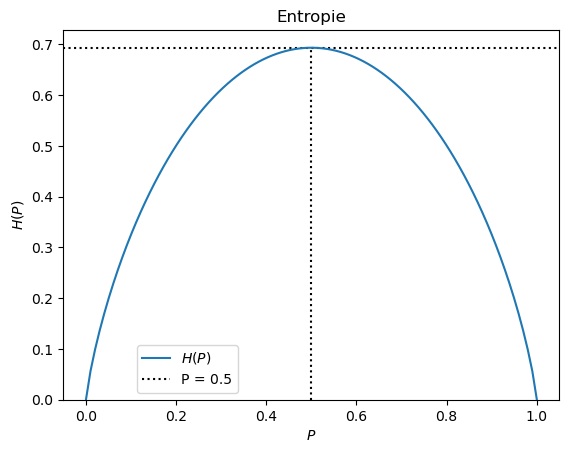
\includegraphics[width=1.0\linewidth]{Images/entropie}
				\label{fig:entropie}
			\end{figure}			
		\end{column}
		\begin{column}{0.5\textwidth}
			Dans le tracé ci-contre:
			\begin{itemize}
				\item On voit que l'entropie atteint une valeur maximale quand la pièce est parfaitement équilibrée: $P = 0.5$.
				\item On voit aussi que l'entropie devient nulle quand la surprise est nulle: $P = 0$ ou $P = 1$.
			\end{itemize}
		\end{column}
	\end{columns}	
\end{frame}

\subsection[Entropie croisée]{Entropie croisée}

\begin{frame}{Intuition de l'entropie croisée}
	Faisons une autre expérience. Je dispose d'une pièce mais vous ne connaissez pas la probabilité réelle $P(X = \text{"Pile"})$. Je vous affirme que la probabilité d'obtenir "Pile" est 0.7. Je note cette probabilité $Q(X = \text{"Pile"}) = 0.7$, c'est l'information que je vous ai communiquée:
	\pause
	\begin{itemize}
		\item J'effectue un lancé avec cette pièce et le résultat est "Pile".
		\item Maintenant vous savez calculer la surprise associée à ce résultat:
		\begin{equation*}
			I(X = \text{"Pile"}) = - \ln{0.7} \approx 0.357
		\end{equation*}
	\end{itemize} 
\end{frame}

\begin{frame}{Intuition de l'entropie croisée}
	\begin{itemize}
		\item Je répète cette expérience plusieurs fois afin que vous puissiez calculer une espérance de la surprise.
		\pause
		\item Mais il y a une différence entre la probabilité \textbf{réelle} d'occurrence d'un lancé aboutissant au résultat "Pile" et la probabilité que vous avez utilisée pour calculer la surprise qui correspond à la probabilité que je vous ai \textbf{communiquée}.
		\pause
		\item Le calcul que vous avez effectué est en fait:
		\begin{equation*}
			\sum_{x \in \{\text{"Pile"}, \text{"Face"}\}} - P(X = x) ln(Q(X = x))
		\end{equation*}
		où $P$ est la probabilité réelle et $Q$ la probabilité communiquée.
	\end{itemize}
\end{frame}

\begin{frame}{Définition de l'entropie croisée}
	\begin{block}{Définition: Entropie croisée}
		On définit l'entropie croisée, notée $H(P, Q)$, entre deux lois de probabilité $P$ et $Q$ comme:
		\begin{equation*}
			H(P,Q) = \mathbb{E}_{X \sim P}\left[I_Q(X)\right] = - \mathbb{E}_{X \sim P}\left[\ln Q(X)\right]
		\end{equation*}
		$P$ représente la probabilité \textbf{réelle} de l'événement $X$ et $Q$ à une loi de probabilité \textbf{estimée}.
	\end{block}
\end{frame}

\begin{frame}{Exemple de calcul de l'entropie croisée}
	Dans l'exemple précédent on a:
	\begin{itemize}
		\item $P(X=\text{"Pile"}) = 0.8$
		\item $Q(X=\text{"Pile"}) = 0.7$
	\end{itemize}
	\pause
	L'entropie croisée se calcule donc comme:
	\begin{equation*}
		\begin{aligned}
			H(P,Q)
			&= - \mathbb{E}_{X \sim P}\left[\ln Q(X)\right] \\
			&= - \sum_{x} P(X = x) \ln{Q(X = x)} \\
			&= - P(X = \text{"P"}) \ln{Q(X = \text{"P"})} - P(X = \text{"F"}) \ln{Q(X = \text{"F"})} \\
			&= - 0.8 \cdot \ln{0.7} - (1 - 0.8) \cdot \ln{(1 - 0.7)} \\
			&\approx 0.526
		\end{aligned}
	\end{equation*}
\end{frame}

\begin{frame}{Tracé graphique de l'entropie croisée}
	\begin{columns}
		\begin{column}{0.5\textwidth}
			\begin{figure}
				\centering
				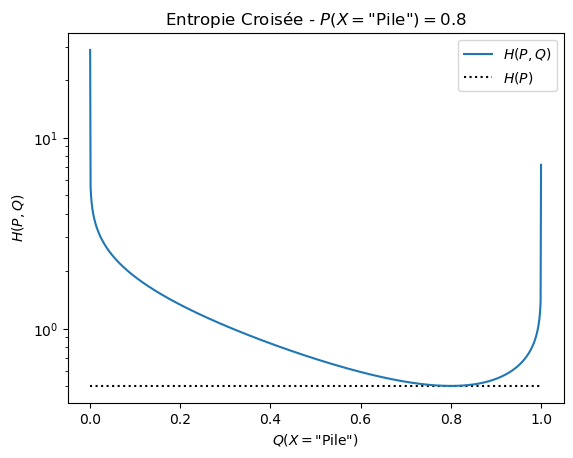
\includegraphics[width=1.0\linewidth]{Images/entropie_croisee}
				\label{fig:entropie_croisee}
			\end{figure}			
		\end{column}
		\begin{column}{0.5\textwidth}
			Dans le tracé ci-contre:
			\begin{itemize}
				\item On voit que l'entropie croisée atteint une valeur minimale quand la probabilité $Q(X = \text{"Pile"}) = P(X = \text{"Pile"})$.
				\item Cette valeur minimale est en fait l'entropie: $H(P,Q) = H(P, P) = H(P)$
			\end{itemize}
		\end{column}
	\end{columns}	
\end{frame}

\begin{frame}{Le passage à l'apprentissage automatique}
	Jusqu'ici, nous avons parlé d'une seule pièce de monnaie. Mais dans un problème de classification (comme prédire si un joueur de rugby est un avant), nous n'avons pas 1 joueur testé $n$ fois, mais bien $n$ joueurs différents.
	\pause
	\vspace{0.3cm}
	C'est comme si nous avions un sac avec \textbf{$n$ pièces de monnaie toutes différentes} (tailles, poids, métaux différents...).
	\pause
	\begin{itemize}
		\item \textbf{Les caractéristiques :} Les propriétés physiques de la pièce $i$ représentent nos variables $X^{(i)}$.
		\item \textbf{La prédiction :} Le modèle observe la pièce $i$ et prédit une probabilité $q^{(i)}$.
		\item \textbf{La réalité :} On lance la pièce $i$ une seule fois, le résultat réel est $y^{(i)} \in \{0, 1\}$.
	\end{itemize}
\end{frame}

\begin{frame}{La surprise pour une pièce spécifique}
	Pour une pièce $i$ donnée de notre jeu de données, nous connaissons déjà le résultat (l'étiquette $y^{(i)} \in \{0, 1\}$).
	\pause
	\begin{itemize}
		\item Puisque le résultat est connu et certain, la probabilité \textbf{réelle empirique} $P$ pour cette pièce est exactement égale à son étiquette $y^{(i)}$.
		\item Le modèle, lui, émet une probabilité \textbf{estimée} $Q$ que l'on note $q^{(i)}$.
	\end{itemize}
	\pause
	\vspace{0.3cm}
	On peut donc écrire la surprise du modèle pour cette pièce en remplaçant $P$ par $y^{(i)}$ et $Q$ par $q^{(i)}$ :
	\begin{equation*}
		I_Q^{(i)} = - \left[ y^{(i)} \ln(q^{(i)}) + (1 - y^{(i)}) \ln(1 - q^{(i)}) \right]
	\end{equation*}
\end{frame}

\begin{frame}{La fonction de perte}
	Pour évaluer la performance globale de notre modèle sur l'ensemble du sac de pièces, nous calculons sa \textbf{surprise moyenne} sur les $n$ pièces.
	\pause
	L'entropie croisée moyenne, aussi dite entropie croisée empirique ou log-loss, s'écrit alors naturellement :
	\begin{equation*}
		H(P, Q) 
		\approx - \frac{1}{n} \sum_{i=1}^n \left[ y^{(i)} \ln{\left(q^{(i)}\right)} + (1 - y^{(i)}) \ln{\left(1 - q^{(i)}\right)} \right]
	\end{equation*}
	\pause
	Entraîner notre modèle de régression logistique revient à trouver les paramètres qui rendent le modèle \textbf{le moins surpris possible} en moyenne lorsqu'il découvre la réalité de nos $n$ exemples !
\end{frame}

\begin{frame}{Entropie relative}
	\begin{block}{Définition: Entropie relative}
		L'entropie relative, ou divergence de Kullback-Leibler parfois juste abrégée en divergence KL, est la différence entre l'entropie croisée et l'entropie:
		\begin{equation*}
			D_{\text{KL}}(P \parallel Q) = H(P,Q) - H(P)
		\end{equation*}
		Note: cette différence n'est pas symétrique:
		\begin{equation*}
			D_{\text{KL}}(P \parallel Q) \ne D_{\text{KL}}(Q \parallel P)
		\end{equation*}
	\end{block}
\end{frame}

\begin{frame}{Entropie relative}
	\begin{itemize}
		\item \textbf{L'entropie}: mesure l'entropie intrinsèque de l'individu.
		\item \textbf{L'entropie croisée}: ajoute une entropie supplémentaire liée à une mauvaise estimation à l'entropie intrinsèque.
		\item \textbf{La divergence KL}: mesure seulement l'entropie supplémentaire liée à la mauvaise estimation.
	\end{itemize}
	\pause
	\vspace{0.5cm}
	Même si on n'utilise pas la divergence KL nominativement, chercher un minimum d'entropie croisée (ou un maximum de log-vraisemblance) dans une problème de classification revient en fait à chercher un modèle qui rend la divergence KL aussi proche possible de 0. C'est donc un concept fondamental en apprentissage automatique.
\end{frame}

\begin{frame}{Résumé: entropie, entropie croisée, entropie relative}
	\begin{itemize}
		\item \textbf{L'entropie}: est le concept fondamental au cœur des arbres de décision.
		\item \textbf{L'entropie croisée}: découle naturellement de l'entropie lorsque la surprise est calculée avec une probabilité estimée plutôt que la probabilité réelle. Cela nous a permis de faire le lien avec la fonction de perte de la régression logistique, qui sera aussi la fonction de perte des réseaux de neurones pour les problèmes de classification.
		\item \textbf{La divergence KL}: mesure spécifiquement l'entropie ajoutée à cause de l'estimation de la probabilité. On l'utilisera également dans le cours des réseaux de neurones sous forme d'une pénalité à la fonction de perte.
	\end{itemize}
\end{frame}